% ---- ETD Document Class and Useful Packages ---- %
\documentclass{ucetd}
%\usepackage{oneinchmargins}
\usepackage{times}
\usepackage{relsize}
\usepackage{enumerate}
\usepackage{graphicx}
\usepackage{url}
%\usepackage{color}
\usepackage[usenames,dvipsnames]{xcolor}
%\usepackage[pagebackref]{hyperref}
%\usepackage[bookmarks=false]{hyperref}

%\hypersetup{colorlinks=true,citecolor=OliveGreen,linkcolor=Maroon,urlcolor=NavyBlue}

%\hypersetup{colorlinks=true,
%citecolor=Maroon,
%linkcolor=Green,
%urlcolor=Maroon}

%\usepackage{breakurl}
\usepackage{setspace}
\usepackage{rotating}

\usepackage{floatflt}
\usepackage{wrapfig}
\usepackage{alltt}
\usepackage{epstopdf}
\usepackage{subfigure}

%\usepackage{listings}
%\usepackage{algorithm}
%\usepackage{algorithmic}

\usepackage{fancyvrb}
%\usepackage{ulem} % for strike out,  
% \em and \sout are now strikes, use \it for italic
% never do this because now all 
\renewcommand{\ttdefault}{cmtt}

%\usepackage{colortbl} % for table color
%\usepackage{pstricks} % for gray hline
%\input{colortab} % for gray hline (must include pstricks)
%\usepackage{array}



% make sure url bib break point does not
% give undefull hbox message and the break line 
% is really nice now
\usepackage{etoolbox}
\apptocmd{\thebibliography}{\raggedright}{}{}


% -----------------------------------------------------
\usepackage{rotating}

\usepackage{subfigure,epsfig,amsfonts}
\usepackage{natbib}
\usepackage{amsmath}
\usepackage{amssymb}
\usepackage{amsthm}


% ---------------------------------------------
% name abbrvs .. 
% ---------------------------------------------
\newcommand{\infokernel}{\mbox{infokernel}}
\newcommand{\unix}{{\sc Unix}}
\newcommand{\dare}{DARE}
\def \samc {\textsc{SamC}}
\def \sampro {\textsc{SamPro}}
\def \samzoo {\textsc{SamZoo}}
\def \sammr {\textsc{SamMr}}
\def \sammace {\textsc{SamMace}}
\def \samcass {\textsc{SamCass}}
\def \sameiger {\textsc{SamEiger}}
\def \modist {\textsc{Modist}}
\def \macemc {\textsc{MaceMC}}
\def \setsudo {\textsc{Setsudo}}
\def \prefail {\textsc{PreFail}}

\def \fate {\textsc{Fate}}
\def \late {\textsc{Late}}
\def \lights {\textsc{LigHTS}}

\def \phi {$\Phi$\xspace}

\def \taxdc {TaxDC}
\def \tdc {TaxDC}
\def \sck {\textsc{SCk}\xspace}
\def \cdb {\textsc{CbsDB}}
\def \cbs {CBS}

\def \prx {\textsc{PilRx}\xspace}

\newcommand{\ts}[1]{{\tt{\small#1}}}


\def \uuu {\textbf{\textcolor{Maroon}{\textbf{$\uparrow$}}}}
\def \uu {\textbf{\textcolor{Maroon}{\textbf{$\Uparrow$}}}}
% \def \nu {\textbf{\textcolor{Maroon}{\textbf{$\nearrow$}}}} % submission only

\def \sleep {\ts{sleep()}}

\newcommand{\num}[1]{\textcolor{red}{\textbf{#1}}}
\def \numOldDeepBugs {12} 
\def \numZkDeepBugs {7}   
\def \numMrDeepBugs {3}
\def \numCsDeepBugs {2}
\def \numZkNewBugs {1}
\def \numMrNewBugs {1}
\def \numNewBugs {2}
\def \numVersions {10}
\def \numLinesSamPro {10,886}
\def \numProtocols {7}
\def \numLinesRule {35}  
\def \numMaxBugSpeedUp {271x}  
\def \numAvgBugSpeedUp {33x}    
\def \numAvgExecTime {40}

\def \numMinRedRatio {37x}  
\def \numMaxRedRatio {166x}  
\def \numRedRatioExecs {3000}

%\newcommand{\mrb}[1]{MR-#1}
%\newcommand{\zkb}[1]{ZK-#1}
%\newcommand{\zk}[1]{ZooKeeper-#1}
%\newcommand{\mr}[1]{MapReduce-#1}
%\newcommand{\cs}[1]{Cassandra-#1}

\newcommand{\jira}[3]{\href{http://issues.apache.org/jira/browse/#1-#3}{#2-#3}}

\newcommand{\mrb}[1]{\jira{MAPREDUCE}{MR}{#1}}
\newcommand{\zkb}[1]{\jira{ZOOKEEPER}{ZK}{#1}}
\newcommand{\cab}[1]{\jira{CASSANDRA}{CA}{#1}}
\newcommand{\hbb}[1]{\jira{HBASE}{HB}{#1}}
\newcommand{\hdb}[1]{\jira{HDFS}{HD}{#1}}
\newcommand{\zk}[1]{\jira{ZOOKEEPER}{ZK}{#1}}
\newcommand{\mr}[1]{\jira{MAPREDUCE}{MR}{#1}}
\newcommand{\ca}[1]{\jira{CASSANDRA}{CA}{#1}}
\newcommand{\hb}[1]{\jira{HBASE}{HB}{#1}}
\newcommand{\hd}[1]{\jira{HDFS}{HD}{#1}}


\def \ll {\ts{L}}
\def \ff {\ts{F}}
\def \pri {\ts{pr}$_{i}$}
\def \prone {\ts{pr}$_{1}$}
\def \prtwo {\ts{pr}$_{2}$}
\def \prtri {\ts{pr}$_{3}$}

\def \ls {\ts{ls}}
\def \als {\ts{als}}
\def \rals {\ts{rals}}
\def \ralsi {\ts{rals}$_{i}$}
\def \ralsone {\ts{rals}$_{1}$}
\def \ralstwo {\ts{rals}$_{2}$}
\def \ralstri {\ts{rals}$_{3}$}
\def \rags {\ts{rags}}


\def \gs {\ts{gs}}
\def \ags {\ts{ags}}
\def \nn {\ts{N}}
\def \none {\ts{N1}}
\def \ntwo {\ts{N2}}
\def \ntri {\ts{N3}}
\def \nfour {\ts{N4}}
\def \mone {\ts{m}$_{1}$}
\def \mn {\ts{m}$_{n}$}
\def \mm {\ts{m}}
\def \fone {\ts{F1}}
\def \ftwo {\ts{F2}}
\def \ftri {\ts{F3}}
\def \ma {\ts{a}}
\def \mb {\ts{b}}
\def \mc {\ts{c}}
\def \md {\ts{d}}
\def \mx {\ts{m1}}
\def \my {\ts{m2}}
\def \xx {\ts{X}}
\def \pg {\ts{pg}}
\def \pl {\ts{pl}}
\def \pp {\ts{p}}
\def \pd {\ts{pd}}
\def \pi {\ts{pi}}
\def \pm {\ts{pm}}
\def \pc {\ts{pc}}

% ---------------------------------------------
% spaces
% ---------------------------------------------
\newcommand{\vtwenty}{\vspace{20pt}}
\newcommand{\vfifteen}{\vspace{15pt}}
\newcommand{\vten}{\vspace{10pt}}
\newcommand{\vfive}{\vspace{5pt}}
\newcommand{\vthree}{\vspace{3pt}}

\newcommand{\vmintwo}{\vspace{-2pt}}
\newcommand{\vminthree}{\vspace{-3pt}}
\newcommand{\vminfive}{\vspace{-5pt}}
\newcommand{\vminten}{\vspace{-10pt}}
\newcommand{\vminfifteen}{\vspace{-15pt}}
\newcommand{\vmintwenty}{\vspace{-20pt}}

% ---------------------------------------------
% overloaded commands
% ---------------------------------------------
\newcommand{\ub}[1]{\underline{{\bf #1}}}
\newcommand{\bquote}{\vspace{-0.25cm} \begin{quote}}
\newcommand{\equote}{\end{quote}\vspace{-0.2cm} }
\def \sec {Section }
\def \yes {$\surd$}

\def \nospace {
  \setlength{\itemsep}{0pt}
  \setlength{\parskip}{0pt}
  \setlength{\parsep}{0pt}
}


\newcommand{\supsection}[1]{\noindent{\Large{\bf #1}}\vten}

\newenvironment{enumerate2}{
  \begin{enumerate}
  \setlength{\itemsep}{1pt}
  \setlength{\parskip}{0pt}
  \setlength{\parsep}{0pt}
}{
  \end{enumerate}
}

\newenvironment{itemize2}{
  \begin{itemize}
 \renewcommand{\labelitemi}{-}
  \setlength{\itemsep}{1pt}
  \setlength{\parskip}{0pt}
  \setlength{\parsep}{0pt}
}{
  \end{itemize}
}

% \renewcommand\thesection{\Alph{section}}



% ---------------------------------------------
% note
% ---------------------------------------------
\newcommand{\hsg}[1]{\textcolor{red}{{\small {\bf (HSG: #1)}}}}
\newcommand{\tl}[1]{\textcolor{red}{{\small {\bf (TL: #1)}}}}
\newcommand{\pj}[1]{\textcolor{red}{{\small {\bf (PJ: #1)}}}}
\newcommand{\thanh}[1]{\textcolor{red}{{\small {\bf (THANH: #1)}}}}
\newcommand{\todo}[1]{\textcolor{red}{{\small {\bf (TODO: #1)}}}}
%\newcommand{\newtext}[1]{\textcolor{blue}{#1}}
\newcommand{\newtext}[1]{#1}
\newcommand{\bluetext}[1]{\textcolor{blue}{#1}}
\newcommand{\rbt}[1]{\textcolor{red}{\textbf{#1}}}
\newcommand{\notes}[1]{\textcolor{darkgray}{
{\footnotesize {\em (Notes: #1)}}}}






% ---------------------------------------------
% bullets
% ---------------------------------------------
\def \vvvnb {\vfifteen \noindent $\bullet$~}
\def \vvnb {\vten \noindent $\bullet$~}
\def \vnb {\vfive \noindent $\bullet$~}

\def \tb {\vspace{8pt}\nb}

\def \vvn {\vten \noindent}
\def \vn {\vfive \noindent}
\def \nb {\noindent $\bullet$~}
\def \ni {\noindent}



% ---------------------------------------------
% counters, steps, hypothesis, tasks
% ---------------------------------------------
\newcommand{\hypo}[1]{
\begin{quote}
\stepcounter{HYPO}{\bf Hypothesis \arabic{HYPO}:} 
{\em #1}
\end{quote}
}

\newcommand{\taskformat}[2]{#1\textsc{#2}}

\newcommand{\task}[3]{
\begin{quote}
\phantomsection
\hypertarget{task#1#2}{}
{\bf Task \taskformat{#1}{#2}:} 
{\em #3}
\end{quote}
}

\newcommand{\tasklink}[2]{\hyperlink{task#1#2}{\taskformat{#1}{#2}}}

\newcounter{HYPO}
\newcounter{TASK}

\newcommand{\rs}{{ResearchStaff$_1$}}
\newcommand{\raOne}{{\bf RA$_1$}}
\newcommand{\raTwo}{{\bf RA$_2$}}
\newcommand{\ndv}{{\bf NDV}}
\newcommand{\ug}{{\bf Undergrad$_1$}}


% ---------------------------------------------
% extra sections, pages
% ---------------------------------------------

\newcommand{\sssubsection}[1]{\vten\textbf{\large{\textsc{#1}}}}


\newcommand{\emptypage}{
\newpage
\thispagestyle{empty}
(empty page)
}


% ---------------------------------------------
% figs
% ---------------------------------------------
\newcommand{\myrotate}[1]{\begin{rotate}{90} {\bf #1} \end{rotate}}

\newcommand{\mycaption}[4][]{%
\ifthenelse{\equal{#1}{}}{
\begin{spacing}{0.95}
\caption{
\label{#2}
{\bf #3. } 
{\em #4}
}
\end{spacing}
}{
\begin{spacing}{0.95}
\caption[#1]{
\label{#2}
{\bf #3. } 
{\em #4}
}
\end{spacing}%
}}


% ---------------------------------------------
% general
% ---------------------------------------------
\newcommand{\eg}{\textit{e.g.}}
\newcommand{\ie}{\textit{i.e.}}
\newcommand{\etal}{\textit{et al.}}
\newcommand{\etc}{etc.}


\newcommand{\symstar}{$^{*}$}
\newcommand{\symtwostars}{$^{**}$}
\newcommand{\symthreestars}{$^{***}$}
\newcommand{\symdag}{$^{\dag}$}
\newcommand{\symddag}{$^{\ddag}$}


% ---------------------------------------------
% counters (\xxx\ cannot appear under figure caption)
% ---------------------------------------------
%\newcommand{\xxx}{{\bf XXX}} % --- no counter 
\newcounter{Xcounter}
\newcommand{\xxxreset}{\setcounter{Xcounter}{1}}
\newcommand{\xxx}{\textcolor{red}{\textbf{XXX$_{\arabic{Xcounter}}$}\stepcounter{Xcounter}}}

% settings
%\relscale{0.97}
%\setlength\parindent{0pt}
%\setlength\parskip{3pt}

\definecolor{fgray}{gray}{0.9}

%\newcommand{\hb}[1]{\jira{HBASE}{h}{#1}}
%\newcommand{\ca}[1]{\jira{CASSANDRA}{c}{#1}}

\newcounter{Fcounter}
\newcommand{\freset}{\setcounter{Fcounter}{1}}

\newcommand{\finding}[1]{
\begin{spacing}{1}
\findingTable{#1}
\end{spacing}
}

\newcommand{\findingTable}[1]{
%\vminfive
\begin{table}[h!]
\begin{center}
\begin{tabular}{|p{5in}|}
\hline
\rowcolor{fgray}
\findingBody{#1}\\
\hline
\end{tabular}
\end{center}
\end{table}
\vminfifteen
\vminfifteen
}

\newcommand{\findingBody}[1]{
\vfive
\begin{spacing}{1.5}
\textbf{Finding \#$\arabic{Fcounter}$:}
\stepcounter{Fcounter}
%\textit{#1}
#1 
\end{spacing}
\vminfifteen
}

\setcounter{Fcounter}{1}

\def \vvni {\vten \noindent}
\def \vni {\vfive \noindent}

\newcommand{\fev}[1]{\textcolor{Maroon}{\textit{#1}}}
\newcommand{\ev}[1]{\textcolor{gray}{\textbf{#1}}}

\newcommand{\bugbox}[1]{
\fbox{
\begin{minipage}{\textwidth}
\vspace{10pt}
\begin{quote}
#1
\end{quote}
\vspace{10pt}
\end{minipage}
}
}

%\newcommand{\codebox}[1]{
%\begin{table}[h!]
%\begin{center}
%\begin{tabular}{|p{3.5in}|}
%\hline
%\begin{spacing}{1.5}
%\vminfifteen
%\begin{alltt}
%#1
%\end{alltt} 
%\vminfifteen
%\vminfifteen
%\vminten
%\end{spacing} \\
%\hline
%\end{tabular}
%\end{center}
%\end{table}
%}

\newcommand{\hmina}{\hspace{-0.05in}}
\newcommand{\hminb}{\hspace{-0.2in}}


% pct prefix means percentage

% num prefix means total number

% MANUAL means manual approach to get the number

% AUTO means, we need to run the script in last minute to get
% the right number



% ================ BAR CHART LABELS (NOT NUMBERS) ==================

% timing conditions (section 3.1) -- TMC
\def \BTMC {\textsf{TC}} % a  -- 4 sub-bars as in Table 2

% input preconditions (section 3.2) -- IP
\def \BFLT  {\textsf{FLT}}  % b 
\def \BTO   {\textsf{TO}}   % c 
\def \BCR   {\textsf{CR}}   % d 
\def \BRB   {\textsf{RB}}   % e 
\def \BPROT {\textsf{PR}} % f 
\def \BBFG  {\textsf{B/F}} % g 

% triggering scope (section 3.3) -- TS
\def \BTSM {\textsf{TS-MSG}} % h 
\def \BTSN {\textsf{TS-ND}} % i 
\def \BTSP {\textsf{TS-PR}} % j 
\def \BTSU {\textsf{TS-UEv}} % k

% error (section 4.1) -- ERR
\def \BERR  {\textsf{ERR}}  % l -- 7 sub-bars as in Table 3
\def \BLG   {\textsf{ER-L/G}}  % m -- see protErrLoc vs. protErrGloba below
\def \BES   {\textsf{ER-E/S}}  % n -- see protErrExp vs. protErrImp below

% failure (section 4.2) -- FAIL
\def \BFAIL {\textsf{FAIL}} % o

% fix -- FIX
\def \BFIX  {\textsf{FIX}}  % p -- 3 sub-bars, FixTime, FixHandEasy, FixHandOt

% other stat -- WHR
\def \BWHR  {\textsf{WHR}}  % q -- 3 sub-bars FIELD, TEST, N/D

\def \B {\textsf{x}}

\def \Bx {\textsf{x}}




% ========================== MANUAL =========================

\def \numTotJiraIss {36,972}  % Hadoop, MapReduce, Yarn, HBase, ZK, Cass
\def \numDcBugs {104}      % total bugs we study
\def \numDcCA {19}
\def \numDcHB {30}
\def \numDcMR {36}
\def \numDcZK {19}

\def \numTagsAll {2,083}
\def \numDescLOC {4,528} % 4-indent space total 


\def \pctx {\xxx\%}
%\def \pctTrigAtom {\xxx\%}




% ===================== FROM AUTO TEX FILE ========================
% the numbers are from auto-generated tex file from stat.py which we can
% manually verify 

\def \totProtCA  {10} % number of unique-protocol-names in CA
\def \totProtHB  {13} % number of unique-protocol-names in HB
\def \totProtMR  {10} % number of unique-protocol-names in MR
\def \totProtZK  {6} % number of unique-protocol-names in ZK
\def \totProtAll {39} % number of unique-protocol-names total

\def \pctFaultYes {63\%}  % fault-* exists
\def \pctFaultTwo {35\%}  % fault-* >= 2
\def \pctFaultThree {12\%}  % fault-* >= 3

\def \pctProtMany {80\%}  % sum-prot >= 2
\def \pctProtTwo {29\%}  % sum-prot == 2
\def \pctProtThree {24\%}  % sum-prot == 3
\def \pctProtFour {8\%}  % sum-prot == 4

\def \pctProtBg {81\%} % at least one protocol is background (BG or Mix)

% trigger: total should be (a bit over) 100% (section 3)
\def \pctTrigOrder  {44\%} % only order
\def \pctTrigAtom   {20\%} % only atom
\def \pctTrigFR     {32\%}  % trigFault + trigReboot
\def \pctTrigMix    {4\%}  % have trigMsg And trigF/R

\def \pctTrigFault  {22\%}
\def \pctTrigReboot {12\%}

\def \pctTrigMsgOrder {69\%} % trigOrder / (trigOrder + trigAtom)
\def \pctTrigMsg    {64\%}  % trigOrder + trigAtom



% ...
\def \pctTrigScopeUnEvOne  {92\%}  % 


% error: total must be 100% (section 4.1)
\def \pctErrLocMem    {5\%} % 
\def \pctErrLocSem    {19\%} % 
\def \pctErrLocHang   {9\%} % 
\def \pctErrLocSil    {13\%} % 
\def \pctErrGlobWrong {29\%} % 
\def \pctErrGlobMiss  {9\%} % 
\def \pctErrGlobSil   {16\%} % 
%local explicit errors, should be \pctErrLocMem + \pctErrLocSem
\def \pctErrLocExp    {23\%} %

% local vs global (derived from above metrics)
\def \pctErrLoc       {46\%} % Loc*
\def \pctErrGlob      {54\%} % Glob*

% explict vs implicit (derived from above metrics)
\def \pctErrExp       {53\%} % LocMem + LocSem + GlobWrong
\def \pctErrImp       {47\%} % LocHang + LocSil + GlobMiss + GlobSil


% failure: total must be 100% (section 4.2)
\def \pctFailOp    {47\%} % i-opfail
\def \pctFailNode  {17\%} % i-down
\def \pctFailData  {28\%} % i-loss + i-corrupt + i-stale
\def \pctFailPer   {8\%} % i-perf





% fix types (total should be 100%)
\def \pctFixTime     {30\%}  % FixMsgTime* + FixFaultTime*
\def \pctFixHandEasy {40\%}  % MsgRet + MsgIgn + MsgAcc + FaultCancel
\def \pctFixHandOth  {30\%}  % 100% - (the two metrics above)



% other statistics (Section 7)
\def \stepMin  {4}
\def \stepTFP  {7}
\def \stepMed  {9}
\def \stepAvg  {10}
\def \stepSFP  {11}
\def \stepMax  {40}

\def \locMin  {1}
\def \locTFP  {44}
\def \locMed  {172}
\def \locAvg  {1,066}
\def \locSFP  {776}
\def \locMax  {28,843}

\def \ttrMin  {0}
\def \ttrTFP  {4}
\def \ttrMed  {14}
\def \ttrAvg  {67}
\def \ttrSFP  {48}
\def \ttrMax  {1,121}

\def \commMin  {1}
\def \commTFP  {12}
\def \commMed  {18}
\def \commAvg  {28}
\def \commSFP  {33}
\def \commMax  {168}

\def \pctWhrField  {46\%}
\def \pctWhrTest   {10\%}
\def \pctWhrNotDef {44\%}



% ======================== IGNORE FROM NOW ==================







% ======================== DEPRECATED ==================


\def \pctPlaneCtl {\xxx\%}

% fix (section 5.1), total is NOT 100%
\def \pctFixMsgTimeGlob {\xxx\%}  % 
\def \pctFixMsgTimeLoc  {\xxx\%}  % 
\def \pctFixMsgHandRet  {\xxx\%}  % 
\def \pctFixMsgHandIgn  {\xxx\%}  % 
\def \pctFixMsgHandAcc  {\xxx\%}  % 
\def \pctFixMsgHandOth  {\xxx\%}  % 

% fix (section 5.2), total is NOT 100%
\def \pctFixFaultTimeGlob {\xxx\%}  % 
\def \pctFixFaultTimeLoc  {\xxx\%}  % 
\def \pctFixFaultHandTO   {\xxx\%}  % 
\def \pctFixFaultHandMsg  {\xxx\%}  % 
\def \pctFixFaultHandCS   {\xxx\%}  % 
\def \pctFixFaultHandOth  {\xxx\%}  % 


% ========================== MESSAGE MACROS =========================


\newcommand \sub[1] {$_{\text{#1}}$}

\def \lbp {{\em b+}}
\def \lcp {c+}
\def \lap {a+}

\def \mm {{\em m}}
\def \mx {{\em x}}
\def \my {{\em y}}
\def \mxy {{\em xy}}

\def \mab {{\em ab}}
\def \mac {{\em ac}}
\def \mbc {{\em bc}}
\def \mcb {{\em cb}}
\def \mca {{\em ca}}
\def \mba {{\em ba}}
\def \mbd {{\em bd}}
\def \mcd {{\em cd}}

\def \sa {S$_1$}
%\def \sb {S$_2$}
\def \sc {S$_3$}
\def \sx {S$_x$}
\def \saa {A$_1$}
\def \sba {B$_1$}
\def \sbr {B$_r$}

\def \ss {$/$}

\def \nt {N$_T$}

\def \ua {$_1$}
\def \ub {$_2$}


\def \spone {$^{1}$}

\def \spa {$^{[a]}$}
\def \spb {$^{[b]}$}
\def \spc {$^{[c]}$}
\def \spd {$^{[d]}$}
\def \spe {$^{[e]}$}
\def \spf {$^{[f]}$}
\def \spg {$^{[g]}$}
\def \sph {$^{[h]}$}
\def \spi {$^{[i]}$}
\def \spj {$^{[j]}$}
\def \spk {$^{[k]}$}
\def \spl {$^{[l]}$}

\newcommand{\jirafootnote}[3]{\vminten\let\thefootnote\relax\footnote{Section \ref{#1}, Table \ref{#2}: #3}}


\newcommand{\jirafootnotable}[2]{\vminten\let\thefootnote\relax\footnote{Section \ref{#1}: #2}}

% numbers for sck


\def \numStudy {12} % total num bugs study
\def \numEval {7} % total num bugs evaluated

\def \maxCF {512}

\def \cfCass {\xxx}
\def \cfRiak {\xxx}
\def \cfVold {\xxx}

\def \numProt {5}
\def \numProtCass {3}
\def \numProtRiak {1}
\def \numProtVold {1}

\def \numVers {9}
\def \numVersCass {5}
\def \numVersRiak {2}
\def \numVersVold {2}


\def \locParser {1051}

\def \locCassTotal {5108}
\def \locRiakTotal {646}
\def \locVoldTotal {1413}


\def \locCassTool {2308}
\def \locRiakTool {429}
\def \locVoldTool {613}

\def \locCassMod {2874}
\def \locRiakMod {217}
\def \locVoldMod {800}




% bugs we reproduced here:

\def \caone {\cab{6127}\xspace}
\def \catwo {\cab{3831}}
\def \catri {\cab{3881}}
\def \cafour {\cab{5456}}


\def \voldonelink {\href{https://groups.google.com/forum/\#!msg/project-voldemort/3vrZfZgQp2Y/Uqt8NgJHg4AJ}{VO-1212}}
\def \riakonelink {\href{http://lists.basho.com/pipermail/riak-users_lists.basho.com/2011-April/003926.html}{RI-3926}}

\def \voldone {\voldonelink\xspace}
\def \riakone {\riakonelink\xspace}


% other bugs we study here


%\def \caa {\href{https://issues.apache.org/jira/browse/CASSANDRA-3831}{ca3831}}
%\def \cab {\href{https://issues.apache.org/jira/browse/CASSANDRA-3881}{ca3881}}
%\def \cac {\href{https://issues.apache.org/jira/browse/CASSANDRA-5456}{ca5456}}
%\def \cad {\href{https://issues.apache.org/jira/browse/CASSANDRA-6127}{ca6127}}
%\def \cae {\href{https://issues.apache.org/jira/browse/CASSANDRA-6345}{ca6345}}



%\def \cba {\href{https://issues.couchbase.com/browse/NCBC-1040}{cb1040}}
%\def \cbb {\href{https://issues.couchbase.com/browse/MB-8640}{cb8640}}
%\def \cbc {\href{https://issues.couchbase.com/browse/MB-15757}{cb15757}}
%\def \cbd {\href{https://issues.couchbase.com/browse/MB-16807}{cb16807}}


% vd
%\def \vda {\href{https://groups.google.com/forum/\#!msg/project-voldemort/3vrZfZgQp2Y/Uqt8NgJHg4AJ}{vd1212}}
%\def \vdb {\href{http://abc.com}{vd??}}
%\def \vdc {\href{http://abc.com}{vd??}}
%\def \vdd {\href{http://abc.com}{vd??}}

% rk 
%\def \rka {\href{http://lists.basho.com/pipermail/riak-users_lists.basho.com/2011-April/003926.html}{rk3926}}
%\def \rkb {\href{http://lists.basho.com/pipermail/riak-users_lists.basho.com/2012-January/007121.html}{rk7121}}
%\def \rkc {\href{http://abc.com}{rk??}}
%\def \rkd {\href{http://abc.com}{rk??}}

\def \totCass {9\xspace}
\def \totHDFS {13\xspace}
\def \totHBase {10\xspace}
\def \totHadoop {2\xspace}
\def \totRiak {1\xspace}
\def \totVold {1\xspace}
\def \totCouch {5\xspace}
\def \totAll  {41\xspace}

\def \mytitle {Unearthing Dependability Bugs in Cloud-Scale Distributed Systems}
%\usepackage[bookmarks=false]{hyperref}

%% Use these commands to set biographic information for the title page:
%\title{SAMC: Semantic-Aware Model Checking for Fast Discovery of Deep Bugs in Cloud Systems}
\title{\mytitle}
\author{Tanakorn Leesatapornwongsa}
\department{Computer Science}
\division{Physical Sciences}
\degree{Doctor of Philosophy}
\date{2016}

%% Use these commands to set a dedication and epigraph text
%\dedication{Dedication Text}
%\epigraph{Epigraph Text}


\begin{document}
%% Basic setup commands
% If you don't want a title page comment out the next line and uncomment the line after it:
\maketitle
%\omittitle

% These lines can be commented out to disable the copyright/dedication/epigraph pages
%\makecopyright
%\makededication
%\makeepigraph


%% Make the various tables of contents
\tableofcontents
\listoffigures
\listoftables

%\acknowledgments
%This Ph.D. could not be accomplished, if I did not get supports from faculty,
family, and friends, which I would like to thank these individuals here.

The first person I need to thank is my adviser (and of course, also one of the
dissertation committee), Prof. Haryadi Gunawi. He guided me since the beginning
to the end. I have learned a lot from him from ``\textit{how to survive
Ph.D.?}'' to ``\textit{how to find a job?}''. It is my great pleasure to have him
as my adviser (and it is also a great experience to be his \textit{first}
student).

Next, I need to thank the other two committee members, Professor Shan Lu and
Professor Ravi Chugh that kindly help to be my committee. I appreciate their
time and their suggestions on my presentation (which is my job talk). I also had
a chance to work with Prof. Lu in one project which is one part in this
dissertation.  Working with Prof. Lu taught me many great lessons.

I also need to thank my colleagues (aka co-authors), Tiratat Patana-anake,
Mingzhe Hao, Pallavi Joshi, Riza Suminto, Thanh Do, Jeffrey Lukman, Huan Ke,
Cesar Stuardo, Daniar Kurniawan, and Bo Fu for their hard working; thank to
other UCARE students Shiqin Yan, Michael Tong, and Huaicheng Li to make UCARE
group lively; and thank to all my friends, department faculty and staff that
helped me many things when I was working on the dissertation.

And also I want to give big thanks to my family. The first most important one is
my mother, the woman who always supports me throughout my life, without her,
there would not be this Tanakorn. The second one is Louise, my wife; she always
helps and supports me during my hard time. The other three are my lovely
sisters, Fon, Nuch, and Nid; they always make me feel good every time I talk with
them. Lastly, I want to thank my father, a man who is my motivations for many
things including this Ph.D.



\abstract
In the era of cloud computing, users move their data
and computation from local machines to cloud,
thus the services are expected to be 24/7 dependable. Cloud services must be
accessible anytime and anywhere, not lose or corrupt users data, and scale as
user base continues to grow.  Unfortunately, guaranteeing cloud services'
dependability is challenging because these cloud services are backed by large
sophisticated distributed systems such as scalable data stores, data-parallel
frameworks, and cluster management systems. Such cloud-scale distributed systems
remain difficult to get right because they need to address data races among
nodes, complex failures in commodity hardware, tremendous user requests, and
much more. Addressing these cloud-specific challenges makes the systems
more complex and new intricate bugs continue to create dependability problems.

This dissertation tries to answer a vital question of cloud dependability:
``{\em how can we make cloud-scale distributed systems more dependable?}'' We
try to answer this question by focusing on the problems of distributed
concurrency bugs and scalability bugs. We focus on these two problems because
they are novel issues that occur in cloud-scale environment only and not many
works addressing them.

Distributed concurrency bug (DC bug) is one unsolved reliability problem in
cloud systems. DC bugs are caused by non-deterministic order of distributed
events such as message arrivals, machine crashes, and reboots. Cloud systems
execute multiple complicated distributed protocols concurrently. The possible
interleavings of the distributed events are beyond developer's anticipations and
some interleavings might not be handled properly that can lead to catastrophic
failures.
%
To combat DC bugs, we make two contributions. First, we conduct a formal study
on DC bugs to gain foundation knowledge for DC-bug combating research. We study
104 DC bugs from various widely-deployed cloud-scale distributed systems in
many characteristics along several axes of analysis such as the triggering
timing condition, input preconditions, error and failure symptoms, and fix
strategies. We present the first complete taxonomy of DC bugs, \taxdc, along
with many findings on DC bugs that can guide future research.

Second, we advance state of the art of distributed system model checking by
introducing ``{\em semantic-aware model checking}'' (SAMC). Distributed system
model checkers (dmck) are used to test system reliability of real systems.
Existing dmcks however rarely exercise multiple faults due to the state-space
explosion problem, and thus do not address present reliability challenges of
cloud systems in dealing with complex faults. SAMC pushes the boundary of dmcks
by introducing a white-box principle that takes simple semantic information of
the target system and incorporates that knowledge into state-space reduction
policies.  We show that SAMC can find deep bugs one to two orders of magnitude
faster compared to state-of-the-art techniques. 

And for the second aspect of system dependability, we focus on scalability bugs.
Scale surpasses the limit of a single machine in meeting users' increasing
demands for computing and storage. On the negative side, scale creates new
development and deployment issues. Developers must ensure that their algorithms
and protocol designs to be scalable. However, until real deployment takes place,
unexpected bugs in the actual implementations are unforeseen. This new era of
cloud-scale distributed systems has given birth to ``scalability bugs'', latent
bugs that are scale-dependent, and only surface in large scale.

To address scalability bugs, we conduct a study on scalability bugs to
understand how they manifest and what their root causes are, and introduce \sck,
a methodology that enables developers to {\em scale-check} distributed systems
and find scalability bugs economically on one machine. \sck\ helps developers
identify potential buggy code and allows developers to colocate a large number
of nodes to test the potential buggy code without sacrificing accuracy. We
remove a problem of hardware contentions (\ie,\ CPU, memory, and thread) with
four novel strategies, and we successfully integrate \sck\ to Cassandra, Riak,
and Voldemort. With \sck, we achieve a high colocation factor (500 nodes), and
can reproduce six scalability bugs and identify two new hidden bugs.


\mainmatter
\chapter{Introduction}
\label{chp-intro}

%``\textit{Cloud computing}'' has been given many definitions from many companies
and experts \cite{TwentyoneCloudDef, IBMCloudDef, PCMagCloudDef,
Foster+08-CloudAndGrid}. These definitions are different in details, but they
have some common characteristics; they are on-demand internet-based services
that can scale to fit increasing users' requirements, and users pay only for
their use. Cloud computing comes in three models: (1) Software as a Service
(SaaS) which is applications that run on Internet, (2) Platform as a Service
(PaaS) which provide computing environment over internet to run services or
applications, and (3) Infrastructure as a Service (Iaas) which provide computing
resources to build platforms and services.
%
Cloud computing help users (from end users to organizational users) reduce the
capital investment in hardware and can make busisness move faster (\xxx{need
citation}). We see a trend that users are moving their data and computation from
local machines and in-house datacenters to the cloud \cite{AdobeCloudStat,
AWSCustomer, GmailStat, GoogleDriveStat, DropboxStat, FacebookStat} \xxx{add
more citation from scientific world}.

This trend makes client-side software get thinner and more heavily rely on the
capability, reliability, and availability of cloud services, thus the services
are expected to be 24/7 dependable. Cloud services must be accessible anytime
and anywhere and not lose or corrupt users data (reliability), and scale as user
base continues to grow (scalability). 
%
Unfulfilled dependability is costly. Some researchers estimate that 568 hours of
downtime at 13 well-known cloud services since 2007 to 2012 had an economic
impact of more than \$70 million \cite{Essers12-70Million}. Others predict
worse: for every hour it is not up and running, a cloud service can take a hit
between \$1 to 5 million \cite{Linthicum13-InfoworldCostOutages}.

Unfortunately, proving cloud services' dependability is challenging. Behind the
cloud computing, it is backed by large sophisticated distributed software stack
\cite{Burrows06-Chubby, Chang+06-BigTable, Chapin+95-Hive, Corbett+12-Spanner,
DeanGhemawat04-MapReduce, DeCandia+07-Dynamo, Ghemawat+03-GoogleFS,
Hunt+10-ZooKeeperPaper,  Lakshman+09-Cassandra, Melnik+10-DremelInteractive,
Zaharia+12-RDD} that is running on top of large-scale cluster \xxx{citation}.
Such cloud distributed systems remain difficult to get right because they need
to address data races among machines, complex failures that randomly happen,
massive user requests, and much more issues that caused from cloud stack.
Addressing these cloud-specific issues makes the systems getting more complex,
and new intricate bugs continue to happen and create dependability problems.

Data races are a fundamental problem in any concurrent software systems. Unlike
non-distributed software, cloud distributed systems are subject to not only
local concurrency bugs, which basically come from thread interleaving, but also
distributed concurrency bugs, which come from inter-node message interleaving. 
Moreover, cloud hardware is built from commodity hardware that failures can
happen at anytime and can be very complex. The timing of these hardware failures
plus message interleaving makes concurrency bugs in cloud systems more complex.

\xxx{talk about massive user request}

\if 0

As more data and computation move from local to cloud settings, cloud-scale
distributed systems such as scale-out storage systems \cite{Chang+06-BigTable,
DeCandia+07-Dynamo, Ghemawat+03-GoogleFS, Nightingale+12-FlatFDS}, computing
frameworks \cite{DeanGhemawat04-MapReduce, Murray+13-NaiadTimelyDataflow},
synchronization services \cite{Burrows06-Chubby, Hunt+10-ZooKeeperPaper}, and
cluster management services \cite{Hindman+11-Mesos, Kumar+13-Yarn} have become a
dominant backbone for many cloud services. Client-side software is getting
thinner and more heavily relies on the capability, reliability, and availability
of cloud systems. Users demand 24/7 dependability of cloud computing systems.
They must be accessible anytime and anywhere and not lose or corrupt users'
data, which means they must be reliable; they have to provision fast and stable
response time, which means they need stable performance; and while user base
continues growing, they must be scalable also.

Unfulfilled dependability is costly. Some researchers estimate that 568 hours of
downtime at 13 well-known cloud services since 2007 to 2012 had an economic
impact of more than \$70 million~\cite{Essers12-70Million}. Others predict
worse: for every hour it is not up and running, a cloud service can take a hit
between \$1 to 5 million~\cite{Linthicum13-InfoworldCostOutages}.
Unfortunately, such cloud-scale distributed systems remain difficult to get
right. 
%
Cloud-scale distributed systems are getting more and more complex. New intricate
bugs continue to create dependability issues that cause major economic loss.
Guaranteeing dependability has proven to be challenging in these systems
\cite{Gunawi+11-FateDestini, Guo+11-Demeter, Wang+14-Exalt, Yang+09-Modist}.

%\section{Dependability Research}

In this proposal, we attempt to improve dependability of cloud-scale distributed
systems. We are tackling this challenge by answering these 2 questions, (1) What
bugs that harm the dependability?, and (2) how do we test the systems to unearth
these bugs so developers can fix them? 
%
The first question is motivated by that we do not have comprehensive knowledge
about the bugs in distributed systems. There are many bug studies on
single-machine softwares \cite{Jin+12-PerformanceBugs,
Lu+08-ConcurrencyBugStudy, Palix+11-FaultsInLinux,
Sahoo+10-StudyBugsServerSoftware}, yet there are few formal bug studies on
distributed-systems softwares; they did not study in a great number and across
multiple types of systems \cite{Li+13-ScopeBugStudy, Xiao+14-NonDetMR}. We
believe that we need comprehensive understanding about cloud bugs to combat
them.

For the second question, we are motivated by the fact that in the past decade,
systems community has developed many testing techniques
\cite{Gunawi+11-FateDestini, Guo+11-Demeter, Wang+14-Exalt, Yang+09-Modist} to
find bugs in distributed systems, but these techniques still have limitations.
For example, \fate\ \cite{Gunawi+11-FateDestini} tests reliability of systems by
injecting faults, but it does not address concurrency in distributed systems.
\modist, which is a model checker, addresses concurrency, but it cannot work in
reasonable time when injecting multiple faults. Or Exalt, which is a framework
to test scalability, cannot be applied to CPU-intensive systems. 

We choose to start dependability research on two aspects, reliability and
scalability.
%
For reliablity, we find that one unsolved reliability problem in cloud systems
is ``{\em distributed concurrency (DC) bugs}''. DC bugs are caused  by
non-deterministic order of distributed events such as message arrivals, faults,
and reboots. Cloud systems execute multiple complicated distributed protocols
concurrently (\eg, serving users' requests, operating some background tasks, and
combined with untimely hardware failures). The possible interleavings of the
distributed events are not completely envisioned by developers and some
interleavings might not be handled properly. The buggy distributed interleavings
can cause catastrophic failures such as data loss, data inconsistencies and
downtimes. Our effort to tackle reliability issues will concentrate on DC
bugs.

And for scalability, we see that most of the work \cite{Calotoiu+13-ApmScaleBug,
Laguna+15-DebugAtScale, Shudler+15-ExascaleLib, Wang+14-Exalt, Zhou+11-Vrisha,
Zhou+13-Wukong} focuses on the data path, mainly to validate the scalability of
read/write operations (linear throughput or stable latency as the cluster
scales). But scalability correctness however is not merely about the data path.
Distributed systems are full of ``control paths'' such as bootstrapping,
rebalancing, and adding/decommissioning nodes (scaling out/down). These
management protocols must modify cluster-wide metadata that lives in each
node in the system (\eg, ring partition table) to decide how data flows in
the cluster. Unfortunately, control path correctness is often overlooked, so we
aim our attention to ``{\em control-plane scalability bugs}'' in this proposal.

We propose how to further the current testing techniques beyond the limitations
in this proposal. The proposal is arranged in this order: chapter \ref{chp-bg}
explains the problem being solved in detail and discusses related work, chapter
\ref{chp-detail} shows our research in detail, and chapter \ref{chp-con} gives a
conclusion.
%
The proposal is a fusion of our previous work and our on-going work. It includes
cloud bug studies \cite{Gunawi+14-Cbs, Leesatapornwongsa+16-TaxDC},
semantic-aware model checking \cite{Leesatapornwongsa+14-Samc}, and scale check
methodology.

\fi

%
% samc
In this thesis, we present semantic-aware model checking (SAMC;
pronounced ``Sam-C''), a white-box principle that takes simple semantic
information of the target system and incorporates that knowledge in
state-space reduction policies.    In our
observation, existing dmcks treat every target system as a complete
black box, and therefore many times perform message re-orderings and
crash/reboot injections that lead to the same conditions that have
been explored in the past.  These {\em redundant executions} must be
removed significantly to tame the state-space explosion problem.  
We find that simple semantic knowledge can
scale dmck greatly.

% main challenge
The main challenge of SAMC is in defining {\em what} semantic
knowledge can be valuable for reduction policies and {\em how} to
extract that information from the target system.  We find that useful
semantic knowledge can come from {\em event processing semantic}
(\ie, how messages, crashes, and reboots are processed by the
target system).  To help testers extract such information from
the target system, we provide {\em generic event processing patterns},
patterns of how messages, crashes, and reboots are processed by
distributed systems in general.


% policies and users
With this method, we introduce four novel semantic-aware reduction
policies.  First, {\em local-message independence} (LMI) reduces
re-orderings of concurrent intra-node messages.  Second, {\em
crash-message independence} (CMI) reduces re-orderings of crashes
among outstanding messages.  Third, {\em crash recovery symmetry}
(CRS) skips crashes that lead to symmetrical recovery
behaviors.  Finally, {\em reboot synchronization
symmetry} (RSS) skips reboots that lead to symmetrical
synchronization actions.  Our reduction policies are {\em generic};
they are applicable to many distributed systems.  SAMC users
(\ie, testers) only need to feed
the policies with short {\em protocol-specific rules} that
describe event independence and symmetry specific to their target
systems.


% systematic
SAMC is purely systematic; it does not incorporate randomness or
bug-specific knowledge.  Our policies run on top of sound model
checking foundations such as state or architectural
symmetry~\cite{Clarke+98-SymReduct, Prasad+00-SymBasedMc} and
independence-based dynamic partial order reduction
(DPOR)~\cite{Flanagan+05-Dpor, Godefroid+96-Dpor}.  Although these
foundations have been around for a decade or more, its application to
dmck is still limited; these foundations require testers to define
{\em what} events are actually independent or symmetrical.  With SAMC,
we can define fine-grained independence and symmetry.


% c3) integration, and also policies, protocols !!!!!!
We have built a prototype of SAMC (\sampro) from scratch for a total
of \numLinesSamPro\ lines of code.  We have integrated \sampro\ to
three widely popular cloud systems,
ZooKeeper~\cite{Hunt+10-ZooKeeperPaper},
Hadoop/Yarn~\cite{Kumar+13-Yarn}, and
Cassandra~\cite{Lakshman+09-Cassandra} (old and latest stable
versions; \numVersions\ versions in total).  We have run \sampro\
on \numProtocols\ different protocols (leader election, atomic
broadcast, cluster management, speculative execution, read/write,
hinted handoff, and gossiper).  The protocol-specific rules are
written in only \numLinesRule\ LOC/protocol on average.  This shows
the simplicity of applying SAMC reduction policies across different
systems and protocols; all the rigorous state exploration and
reduction are automatically done by \sampro.

% evaluation, 3 crashes, 3 reboots ... 
To show the power of SAMC, we perform an extensive evaluation of
SAMC's speed in finding deep bugs.  We take \numOldDeepBugs\ old
real-world deep bugs that require multiple crashes and reboots (some
involve as high as 3 crashes and 3 reboots) and show that SAMC can
find the bugs 
% up \numAvgBugSpeedUp\ faster on
% to \numMaxBugSpeedUp\ faster (
one to two orders of magnitude faster compared to state-of-the-art
techniques such as black-box DPOR, random+DPOR, and pure random.  We
show that this speed saves tens of hours of testing time.  More
importantly, some deep bugs cannot be reached by non-SAMC approaches,
even after 2 days; here, SAMC's speed-up factor is potentially much
higher.  We also found \numNewBugs\ new bugs in the latest version of
ZooKeeper and Hadoop.


% summarize
To the best of our knowledge, our work is the first solution that
systematically scales dmck with the inclusion of failures.  We believe
none of our policies have been introduced before.  Our prototype is
also the first available dmck for our target systems.  Overall, we
show that SAMC can address deep reliability challenges of cloud
systems by helping them discover deep bugs faster.

% the rest
The rest of the thesis is organized as follows.  First, we present a
background and an extended motivation (\sec\ref{sec-mot}).  Next, we
present SAMC and our four reduction policies (\sec\ref{sec-samc}).
Then, we describe \sampro\ and its integration to cloud systems
(\sec\ref{sec-impl}).  Finally, we close with evaluations
(\sec\ref{sec-eval}), related work (\sec\ref{sec-related}),
conclusion (\sec\ref{sec-conclude}), and future 
work(\sec\ref{sec-future}).



\chapter{Background and Related Work}
\label{chp-bg}

This chapter provides the background of this dissertation. We briefly discuss
about cloud computing and cloud backend in Section \ref{bg-cloud}, cloud bugs
in Section \ref{bg-bugs}, DC bugs in detail in Section \ref{bg-dc}, and
scalability bugs in Section \ref{bg-sc}. 
%
%We also discuss about related work to combat DC bugs and scalability bugs at the
%end of this chapter (Section \ref{bg-related}).

\section{Cloud Computing and Cloud-Scale Distributed Systems}
\label{bg-cloud}

\subsection{Cloud Computing}

In the past decade, \textit{cloud computing} has become widespread buzzword
that IT people often talk about. However, there is few agreement on what it
really means; many companies and experts have given many definitions
\cite{TwentyoneCloudDef, IBMCloudDef, PCMagCloudDef, Foster+08-CloudAndGrid}
that are different in details, but they share some common characteristics: cloud
computing is on-demand internet-based services that can scale to serve growing
users' requests, and users \textit{pay as they go}.

% probably write about 3 models of cloud SaaS, PaaS, IaaS

%benefit of cloud computing
Cloud computing can attract a number of users to move their data and
computation from local machines and private datacenters to the cloud
\cite{AdobeCloudStat, AWSCustomer, GmailStat, GoogleDriveStat, DropboxStat,
AstroInCloud, FacebookStat, Luo+16-BigDataBioResearch}.
It provides many benefits as shown below:
\begin{itemize}
\item Users can access their computing resources and data any time and any
where. For example, Google Doc allows users to create/modify their documents on
one machine and access them later on mobile devices. This advantage also
enables new classes of applications, especially, mobile applications
\cite{DropboxWebsite, GmailWebsite, GoogleDriveWebsite, iCloudWebsite,
SiriWebsite} 

\item Users can cut the cost of hardware investment, but can get immedate access
to computing resources. Moreover, this will help improve hardware utilization
because users do not need to pay while they are not using the resources
\cite{Marston+11-CloudBusiness}.

\item Most importantly, cloud computing help users to scale their services in a
convenient manner. When their workload is growing up, they can just purchase
more computing power from their cloud service providers.
\end{itemize}

\subsection{Cloud-Scale Distributed Systems}

Behind the cloud computing, it is sophisticated distributed systems running on
large-scale clusters. Unlike traditional computing, when the number of users or
workload increase, we do not upgrade hardware specification, but add more
machines to the systems. Thus, cloud-scale distributed systems are designed to
be scalable to handle tremendous users' requests. Moreover, the cluster is
built from commodity machines which hardware failures are not optional and can
be very complex (\eg multiple machine failures, disk failures, and network
partitions), so cloud systems must be able to handle these complex failures
\cite{Abadi09-Cloud, Gunawi+11-FaaS-TR, Hamilton07-Deploying}.  We will discuss
some types of cloud-scale distributed systems below as these systems are
systems that we work on in this dissertation.

\begin{itemize}

\item \textit{Distributed file systems}: these are file systems that stores
files across machines in clusters (however, some systems cannot be mounted as
other traditional file systems, and some users consider them as data store
\cite{HadoopStorage}). Distributed file systems do replication or erasure coding
across machines in order to be fault tolerant, and to increase performance via
data aggregation. Exmaples of these systems are GFS from Google
\cite{Ghemawat+03-GoogleFS}, and HDFS from Apache \cite{Shvachko+10-HDFSPaper}
which is an open-source version of GFS.

\item \textit{Data-parallel framework}: these frameworks process \textit{big
data} by leveraging parallelism. It eases parallel computing by enabling users
to increase computing power by just adding more machines without changing their
programs.  One of well-known data-parallel frameworks is MapReduce from Google
\cite{DeanGhemawat04-MapReduce}.  As its name states, MapReduce is a
programming model that consist of \textit{map} and \textit{reduce} functions.
Map functions process key-value pairs of data and generate intermediate
key-value pairs, which reduce functions will values of data with the same keys.
Apache also has open-source framework, which is similar to Google MapReduce,
called Hadoop MapReduce \cite{HadoopWeb}.

\item \textit{NoSQL data stores}: These are data stores that are not relational
database. Storing and accessing data do not have strict tabular relations like
in relational database, and are not done by SQL query (some systems support SQL
query but not fully), such as key-value stores, document stores, and object
stores. Most NoSQL stores adopt the concept of ``eventual consistency'' to
improve availablity during network partition (favoring ``C'' in CAP theorem). An
example of NoSQL is Dynamo from Amazon \cite{DeCandia+07-Dynamo}. Dynamo is
decentralized distributed key-value store. Its open-source counterpart from
Apache is Cassandra \cite{Lakshman+09-Cassandra}.

\item \textit{Synchronization services}: These are utility services that support
other large distributed systems. They help nodes in other systems synchronize
some metadata such as global locking, configuration maintaining, and naming.
Examples of the synchronization services are Chubby from Google
\cite{Burrows06-Chubby} and ZooKeeper from Apache \cite{Hunt+10-ZooKeeperPaper}.

\end{itemize}
 % talk about cloud-scale distributed systems
\section{Cloud Bugs}
\label{bg-bugs}
 % talk about cloud bugs
\section{Distributed Concurrency}
\label{bg-dc}

\subsection{Local Concurrency and Distributed Concurrency}


\begin{figure}
\bugbox{
{\bf ZooKeeper Bug \#1264:}
\enumerate{
\item \fev{Follower F crashed} in the past,
\item \fev{F reboots} and joins the cluster; then \fev{F synchronizes data} with Leader L
\item F sends FOLLOWERINFO message to L [synchronization message]
\item L sends LEADERINFO message to F [synchronization message]
\item F sends ACKEPOCH message to L [synchronization message]
\item L sends SNAP message to F [synchronization message]
\item L sends data tree snapshot to F [synchronization message]
\item L sends NEWLEADER message to F [synchronization message]
\item \fev{Client C sends a request} to update data with Tx-\#15 to L; L does atomic broadcast to update all followers
\item L sends update proposal message for Tx-\#15 to F [broadcast message]
\item F sends update ack message for Tx-\#15 to L [broadcast message]
\item \fev{L sends update commit message} for Tx-\#15 to F [broadcast message]
\item \fev{F applies the update} for Tx-\#15 to in-memory data tree, but not to on-disk log (because F has not received UPTODATE message)
\item \fev{L sends UPTODATE message} to F [synchronization message]
\item C sends a request to update data with Tx-\#16 to L
\item L sends update proposal for Tx-\#16 to F
\item F sends update ack for Tx-\#16 to L
\item L sends update commit for Tx-\#16 to F
\item F applies the update for Tx-\#16 to in-memory data tree and on-disk log
\item \fev{F crashes} (before \fev{F does snapshot})
\item F reboots and joins the cluster again
\item L synchronized data with F by sending update starting from Tx-\#17
\item F loses the update for Tx-15 C did in step 9
}
}
\mycaption[ZooKeeper-1264 bug]{fig-zk1264}{ZooKeeper-1264 bug}{A concurrency bug in ZooKeeper that
is caused from a mix of untimely message arrivals and crash timing. This bug
surfaces when a follower receives update commit message (step 12) in the middle
of an atomic operation (step 3-14) and the follower crashes before it does
snapshot (step 20)}
\end{figure}


\if 0
\begin{figure}[t]
\centering
%\footnotesize
\begin{tabular}{|p{3.2in}|} 
% ---------------------------------------------------- Sample
\hline
{\bf \zk{1264}:}
\ev{(1)} \fev{Follower F crashed} in the past,
\ev{(2)} \fev{F reboots} and joins the cluster,
\ev{(3)} Leader L sync data with F and send snapshot, 
\ev{(4)} \fev{In the middle of step 3-6},
% Before syncing finishes (in step 6), 
client updates data with Tx-\#15; L forwards the update to F,
\ev{(5)} F applies the update in memory only, due to a concurrent sync,
\ev{(6)} L tells F syncing is finished, % \fev{after step 5},
\ev{(7)} Client updates data with Tx-\#16; F writes update to disk correctly,
\ev{(8)} \fev{F crashes},
\ev{(9)} \fev{F reboots} and joins the cluster again,
\ev{(10)} L sync data with F, but this time L sends only ``diff'' starting with Tx-\#17
\ev{(11)} F permanently \fev{loses data} from Tx-\#15,
inconsistent with L and other followers!
% \ev{(12)} Violaton: permanent data inconsistency as F does not have data from txid \#15,
\\ \hline
% ----------------------------------------------------
\end{tabular}
%---------------------------------
\vminfive
\mycaption{fig-zook}{A DC bug in ZooKeeper}{}
\end{figure}
\fi


A well-known concurrency that developers most familiar with is from thread
execution interleaving in multi-threaded software or what we call in this
dissertation ``local concurrency''. Multi-threaded software has become common in
the age of multi-core processor, however, building multi-threaded software is
hard. Developers need to handle all possible interleaving of multiple threads
that are accessing to same data properly, otherwise concurrency bugs will
happen. These bugs are timing-related and non-deterministic, and they are
extremely difficult to test and debug.

For distributed systems, other than local concurrency, the systems are also
subject to ``distributed concurrency'' that is caused from interleaving of
computations in multiple nodes. Nodes in distributed systems do not have shared
memory and they access data in other nodes via network communication, so
basically, distributed concurrency comes from concurrent message arrivals and
internal computations in running nodes.

Other than timing of message arrivals and local computations, concurrent bugs in
distributed systems are caused from timing of failures as well. Cloud software
is often deploy on commodity hardware for horizontal scaling purpose (Section
\ref{bg-sc-type}). This commodity hardware is unreliable, and hardware failures
are not an option \xxx{citation as Thanh did}. Cloud distributed systems need to
response to these failures, they need to detect and recover from the failures
and makes sure that users's data will not be lost or corrupted. Gauranteeing
this correctness is proven to be hard \xxx{cite FATE, Thanh's disser},
cloud-scale distributed systems need to handle failures that can happen at any
time and at any state of the systems. Some ordering of message arrivals could
make systems into state that developers never anticipate and is prone to error
when failure happens.

Consider hardware failures, concurrency bugs in cloud-scale distributed systems
is not only about interleaving of message arrivals and local computations, but
also timing of hardware failures as well. Figure \ref{fig-zk1264} shows an
example of a concurrency bug that happens because of untimely ordering of
message arrivals and node crashes. This bugs surfaces only if a follower
receives an UPTODATE message (step 14) after a commit message (step 12), and the
follower crashes before it does snapshot (step 20); only untimely message
arrivals or the timing of follower crash is not enough for bug to surface.

\subsection{Distributed Systems Model Checker (DMCK)}
\label{sec-bg-dmck}

In order to unearth DC bugs the question we have to answer is: ``{\em can we
exercise necessary conditions (\ie workloads and faults) and test different
event re-ordering to hit the bugs?}''. This is the job of distributed system
model checkers (dmck), which are gaining popularity recently
\cite{Guo+11-Demeter, Killian+07-LifeDeathMaceMC, Simsa+10-Dbug,
Yang+09-Modist}. Dmck works by intercepting distributed events and permuting
their ordering, and hereby pushing the target system into corner-case situations
and unearthing hard-to-find bugs. However, the more events included, the more
scalability issues will arise due to state-space explosion.




\begin{figure}[t]

\centerline{
%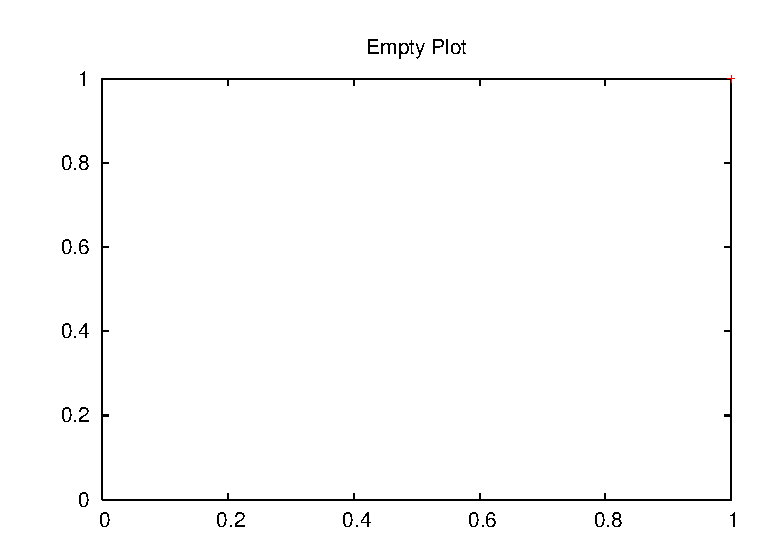
\includegraphics[height=1in]{F/empty.eps}
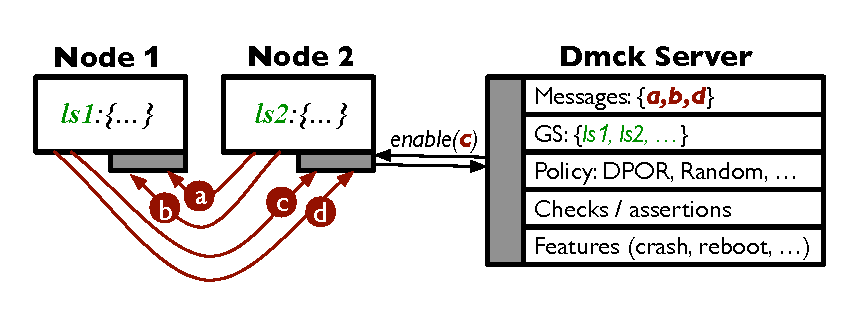
\includegraphics[height=2in]{F/dmck/dmck.eps}
}
\vminfive
\mycaption[Distributed System Model Checker]{fig-dmck}{DMCK}{The figure illustrates a typical framework
of a distributed system model checker (dmck).
}
%\vminten
\end{figure}

\if 0
The figure shows a dmck server model checking
a target distributed system containing two nodes.  
Communications in the target system are interposed 
\fi


The last ten years have seen a rise of software model checker that checks
distributed systems directly at the implementation level.  Figure~\ref{fig-dmck}
illustrates a dmck integration to a target distributed system, a simple
representation of existing dmck frameworks~\cite{Guo+11-Demeter,
Killian+07-LifeDeathMaceMC, Simsa+10-Dbug, Yang+09-Modist}.  The dmck inserts an
interposition layer in each node of the target system with the purpose of
controlling all important events (\eg, network messages, timeouts) and
preventing the target system to process the events until the dmck enables them.
A main dmck mechanism is the permutation of events; the goal is to push the
target system into all possible ordering scenarios.  For example, the dmck can
enforce \ts{abcd} ordering in one execution, \ts{bcad} in another, and so on.

\subsection{Symbolic Execution}
% symbolic execution ...
Symbolic execution is another powerful formal method to verify systems
correctness.  Symbolic execution also faces an explosion problem, specifically
the path explosion problem.  A huge body of work has successfully addressed the
problem and made symbolic execution scale to large (non-distributed) software
systems \cite{Bucur+11-ParallelSymEx, Cadar+08-KLEE, Chipounov+11-S2e,
Cui+13-RuleDirectedSymExec, Zamfir+10-Synthesis}.  Symbolic execution and model
checking can formally be combined into a more powerful
method \cite{Burch+92-SymbolicMC}, however this concept has not permeated the
world of distributed systems; it is challenging to track symbolic values across
distributed nodes.

\subsection{Fault Injector}
% fault injector
Reliability bugs are often caused by incorrect handling of
failures \cite{Gunawi+11-FateDestini, Gunawi+08-EIO}.  Fault-injection testing
however is challenging due to the large number of possible failures to inject.
This challenge led to the development of efficient fault-injection testing
frameworks.  For example, AFEX \cite{Banabic+12-Blackbox} and
LFI \cite{Marinescu+10-ExtensibleLFI} automatically prioritize ``high-impact
targets'' (\eg, unchecked system calls).  These novel frameworks target
non-distributed systems and thus the techniques are different than ours.

% distributed systems
Similarly, recent work highlights the importance of testing faults in cloud
systems (\eg, \fate \cite{Gunawi+11-FateDestini}, \setsudo
\cite{Joshi+13-SetsudoTesting}, \prefail \cite{Joshi+11-PreFail}, and OpenStack
fault-injector \cite{Ju+13-FaultResOpenStack}). However, these frameworks are
not a dmck; they cannot re-order concurrent messages and failures and therefore
cannot catch distributed concurrency bugs systematically.


\section{Scalability}
\label{bg-sc}

\subsection{Vertical Scaling vs Horizontal Scaling} 
\label{bg-sc-type}

When systems' workload grows (the number of users raises or individual users'
requests increase), developers need to scale the systems to add more capability
and keep users satisfied. Two traditional approaches to scale system are used as
we show below \cite{Michael+07-ScaleUpXScaleOut}:
\begin{itemize}

\item \textbf{Vertical scaling or scale-up}: this approach expands system
capabilities by adding more resources (\eg, CPU, memory, and storage) to a
single node to boost its performance, and make software to leverage additional
resources. For example, run more processes of applications in the node.

\item \textbf{Horizontal scaling or scale-out}: this approach enhance the
capability by adding more nodes to current distributed systems to yeild higher
aggregate capability; mostly, the nodes that we are adding are low-cost
machines.

\end{itemize}

In the past, vertical scaling was widely favored by many companies.
Multiprocessor with higher clock rate can satisfy computing power need of
largest companies \cite{Michael+07-ScaleUpXScaleOut}. Vertical scaling requires
less human effort than horizontal scaling; it does not need more administrative
effort because the number of machines and systems administrators need to handle
is still the same. The disadvantages of vertical scaling are the upgradability
is limited by existing hardware manufacturing, and the upgrade cost is
expensive.

Because of the upgradability and price issues, nowadays, the trend goes to
horizontal scaling. Many cloud service companies adopt this approache (\eg,
Google, Facebook, Amazon, \etc). The cost of horizontal scaling is much more
cheaper than the vertical scaling and there is not limitation for hardware to
scale out infinitely (the limitations are posed by software stack)
\cite{ScaleUpVsScaleOut}. In addition, hardware manufaturers try to facilitate
scale-out approach \cite{Michael+07-ScaleUpXScaleOut}.

\subsection{Scalability Testing}

As we discussed in \ref{bg-sc-type}, horizontal scaling or scale-out is a trend
now because it does not expose hardware limitation. The limitation is in
software stack so developers need to invent scalable algorithms and protocols,
however, before real deployment, if they do not have a large cluster to test
their implementations, there could be ``scalability bugs'' hide there.

We now discuss popular approaches (simulation, extrapolation, and emulation) for
unearthing scalability bugs that avoid acquiring a number of machines, because
testing on such deployments is costly.
% ......
First, simulation approaches test system/application models in different scales
\cite{Calotoiu+13-ApmScaleBug, Laguna+15-DebugAtScale}, However, a model can
look scalable but the actual implementation can contain unforeseen bugs. Later
in Section \ref{chp-scb}, we will show our observations from \textit{real world}
scability bugs that simulation cannot detect them.

Second, extrapolation monitors system behaviors in ``mini clusters'' and
extrapolates them to larger scales (\sec2.1 in \cite{Wang+14-Exalt}). However,
mini clusters tend to be order(s) of magnitude smaller than real deployments.
Most importantly, system behaviors do not always extrapolate linearly
\cite{Wang+14-Exalt}. 

Finally, real-scale emulation checks real implementations in an emulated
environment \cite{Gupta+08-DieCast, Wang+14-Exalt}. This approach emulates real
large-scale system in a single machine. For example, a naive way to achieve this
is just colocating multiple processes/VMs on one machine. The limitation here is
emulation consumes real resources (CPU, memory, and storage), so with limited
resources, we can not emulate \textit{really large} deployment (\eg, can test up
to 50-node deployment). Some works try to resolve this resource contention issue
\cite{Gupta+08-DieCast, Wang+14-Exalt}. We will discuss them in related work
(Section \ref{xxx}).

\subsection{Scalability Benchmarking}

Scalability benchmarking (\eg, YCSB~\cite{Cooper+10-YCSB}) is a standard method
to check throughput/latency scalability.  The results are useful for
advertising system capabilities, and thus acquiring a large number of machines
is justifiable.  Debugging code however is a different matter; for every
scalability bug, developers need to debug the code in tens/hundreds of
iterations.  A single-machine debugging approach is valuable.

%\section{Related Work}
\label{bg-related}

\section{Conclusion}

In this chapter, we discuss about cloud-scale distributed systems, software
backend for the cloud computing. We show what the current trend of the systems
is and how they are design. We also discuss about distributed concurrency and
scalability, the two important aspects of cloud-scale distributed systems that
could threaten dependability of the systems. We briefly discuss how system
community address issues from the concurrency and scalability. Unfortunately,
distributed concurrency bugs are still an unsolved problem, and scalability bugs
are novel and not many works address about them.



\chapter{Research Detail}
\label{chp-detail}

To unearth bugs in cloud-scale distributed systems, the first thing we need is
comprehensive knowledge about them, so we can establish proper solutions. In our
research plan, we start with general bug study on cloud systems to see the big
picture of the current problems. Then we dissect DC bugs and scalability bugs to
analyze.
%
For DC bugs, we will advance the state of the art of dmcks. We are introducing 
more pruning policies to tackle state-space explosion problem. And for
scalability bugs, we will fill the missing piece of control-plane protocol bugs
focusing on P2P systems.

\section{Bug Study}

Bug or failure studies can significantly guide many aspects of dependability
research. Many dependability researchers have recently employed formal studies
on bugs and failures \cite{Guo+13-CureIsWorse, Li+13-ScopeBugStudy}. These
studies can identify opportunities for new research, build taxonomies of new
problems, or test new tools. We start our work by doing formal bug study to gain
foundations of bugs in cloud systems.

\subsection{Cloud Bug Study (Prvious Work)}

As an initiative, our group have performed the largest bug study in six
important Apache cloud infrastructures including Cassandra, Flume, Hadoop
MapReduce, HBase, HDFS, and ZooKeeper \cite{Gunawi+14-Cbs}. We reviewed in total
21,399 submitted issues within a three-year period (2011-2014).  We perform a
deep analysis of 3,655 ``vital'' issues (\ie, real issues affecting deployments)
with a set of detailed classifications.  \subsubsection{Methodology}


\begin{table}[!hbt]
\begin{center}
% {\small
\begin{tabular}{r|p{5in}}
\hline
{\bf Classification} & {\bf Labels} \\
\hline
Issue Type & Vital, miscellaneous. \\
\hline
Aspect & Reliability, performance, availability, security, consistency,  scalability, topology, QoS. \\
\hline
Bug scope & Single machine, multiple machines, entire cluster. \\
\hline
Hardware & Core/processor, disk, memory, network, node. \\
\hline
HW Failure & Corrupt, limp, stop. \\
\hline
Software & Logic, error handling, optimization, config, race, hang, space, load. \\
\hline
Implication & Failed operation, performance, component downtime, data loss, data staleness, data corruption. \\
\hline
\end{tabular}


%
\if 0
\begin{tabular}{p{3in}}
\\
\hline
{\bf Per-component Labels} \\
\hline
{\em Cassandra:} Anti-entropy, boot, client, commit log, compaction, cross system, get, gossiper, hinted handoff, IO, memtable, migration, mutate, partitioner, snitch, sstable, streaming, tombstone. \\
\hline
{\em Flume:} Channel, collector, config provider, cross system, master/supervisor, sink, source. \\
\hline
{\em HBase:} Boot, client, commit log, compaction, coprocessor, cross system, fsck, IPC, master, memstore flush, namespace, read, region splitting, log splitting, region server, snapshot, write. \\
\hline
{\em HDFS:} Boot, client, datanode, fsck, HA, journaling, namenode, gateway, read, replication, ipc, snapshot, write. \\
\hline
{\em MapReduce:} AM, client, commit, history server, ipc, job tracker, log, map, NM, reduce, RM, security, shuffle, scheduler, speculative execution, task tracker. \\
\hline
{\em Zookeeper:} Atomic broadcast, client, leader election, snapshot. \\
\hline
\end{tabular}
\fi
%---------------------------------
\end{center}
%\vminfifteen
%\vminten
\vminfive
\mycaption{tab-tag}{Issue Classifications}{
%
%  The tables list our issue classifications
%and per-component labels.
% the raw bug repositories have component labels, but they are
%unsuitable for our study (\eg, they are 
%too coarse-grained,  based on sub-directory names, and often
%do not pinpoint the buggy components).
}
%\vminfifteen
%\vminfive
\end{table}


\begin{itemize}

\item {\bf Target Systems \& Bug Repositories:} We select six popular cloud
systems that represent a diverse set of system architectures: Hadoop
MapReduce~\cite{HadoopWeb} (distributed computing frameworks), Hadoop File
System (HDFS)~\cite{HDFSWeb} (scalable storage systems), HBase~\cite{HBaseWeb}
and Cassandra~\cite{CassandraWeb} (distributed NoSQL systems),
ZooKeeper~\cite{ZooKeeperWeb} (synchronization services), and finally
Flume~\cite{FlumeWeb} (streaming systems).
%
All development projects of the target systems maintain highly organized issue
repositories.
%
Each repository contains development and deployment issues submitted mostly by
the developers or a larger user community. The term ``issue'' is used here to
represent both bugs and new features.

\if 0
For every issue, the repository stores many ``raw'' labels. There are five
options for {\em bug priority} label: trivial, minor, major, critical, and
blocker. We label the first two as ``minor'' and the last three as ``major''.
Although we analyze all issues in our work, we only focus on major issues in
our analysis.
\fi

\item {\bf Issue Classifications:} We introduce issue classifications as
displayed in Table~\ref{tab-tag}. 
%
We carefully read each issue to decide whether the issue is vital. If an issue
is vital we proceed with further classifications, otherwise it is labeled as
miscellaneous and skipped in our study. 

\end{itemize}

\subsubsection{Study Result}

The finding of this study was published in the \cbs\ paper \cite{Gunawi+14-Cbs}.
The product of our classifications is stored in \cdb, a set of raw text files,
data mining scripts and graph utilities \cite{CBS}, which enables us (and other
\cdb\ users) to perform both quantitative and qualitative analysis of cloud
issues. 

This study brings new insights on some of the most vexing problems in cloud
systems. We show a wide range of intricate bugs, many of which are unique to
distributed cloud systems (\eg, scalability, topology, and killer bugs). And it
is the main source of our DC-bug taxonomy and scalability-bug analysis.

\subsection{DC Bug Taxonomy}

While there have been many LC-bug studies, we are not aware of any large-scale
study of DC bugs. To fill the void, we have created the largest and most
comprehensive taxonomy of 104 real-world DC bugs (named \taxdc) from four
distributed system: Cassandra, HBase, Hadoop MapReduce/Yarn, and ZooKeeper
\cite{Leesatapornwongsa+16-TaxDC}.

\subsubsection{Methodology}

\definecolor{Gray}{gray}{0.75}
\begin{table}[!htb]
%\footnotesize
\centering
\begin{tabular}{lp{5.5in}}
\toprule
%\rowcolor{Gray}
\multicolumn{2}{c}{{\bf Triggering} }\\
\midrule
\multicolumn{2}{l}{\it What is the triggering timing condition?}\\
&{Message arrives unexpectedly late/early}\\
&{Message arrives unexpectedly in the middle}\\
&{Fault (component failures) at an unexpected state}\\
&{Reboot at an unexpected state}\\
\multicolumn{2}{l}{\it What are the triggering inputs preconditions?}\\
 & {Fault, reboot, timeout, background protocols, and others}\\ 
%&{\scriptsize Node/Job crash}\\
%&{\scriptsize Node/Job restart after crash}\\
%&{\scriptsize Node/Job shut-down}\\
%&{\scriptsize Node/Job start-up}\\
%&{\scriptsize Time out}\\
%&{\scriptsize Others (e.g., client requests)}\\
\multicolumn{2}{l}{\it What is the triggering scope?}\\
&{\it How many nodes/messages/protocols are involved?}\\
\midrule
%\rowcolor{Gray}
\multicolumn{2}{c}{{\bf Errors \& Failures} }\\
\midrule
\multicolumn{2}{l}{\it What is the error symptom?}\\
&{Local memory exceptions}\\
&{Local semantic error messages \& exceptions}\\
&{Local hang}\\
&{Local silent errors (inconsistent local states) }\\
&{Global missing messages}\\
&{Global unexpected messages}\\
&{Global silent errors (inconsistent global states)}\\
\multicolumn{2}{l}{\it What is the failure symptom?}\\
&{Node downtimes, data loss/corruption, operation failures, slowdowns}\\
\midrule
%\rowcolor{Gray}
\multicolumn{2}{c}{{\bf Fixing} }\\
\midrule
\multicolumn{2}{l}{\it What is the fix strategy?}\\
&{Fix Timing: add global synchronization}\\
&{Fix Timing: add local synchronization}\\
&{Fix Handling: retry message handling at a later time}\\
&{Fix Handling: ignore a message}\\
&{Fix Handling: accepting a message without new computation logics}\\
&{Fix Handling: others}\\
\bottomrule
\end{tabular}
\mycaption{tab:tax}{Taxonomy of DC Bugs}{}
\end{table}


\begin{itemize}

\item {\bf Target Systems \& Bug Repositories:} We examined bugs from four
distributed systems that represent a diverse set of system architectures: Hadoop
MapReduce \cite{HadoopWeb} (distributed computing frameworks), HBase
\cite{HBaseWeb} and Cassandra \cite{CassandraWeb} (distributed NoSQL systems),
and ZooKeeper \cite{ZooKeeperWeb} (synchronization services).
%
We started our study from \cdb \cite{CBSWeb}, which already labels issues
related to concurrency bugs. However, beyond simple labeling, the \cbs work does
not differentiate DC from LC bugs and did not dissect DC bugs further.
Thus, we first filtered out LC bugs, then exclude DC bugs that do not contain
clear description, and finally randomly picked \numDcBugs\ samples from the
remaining detailed DC bugs, specifically \numDcCA\ Cassandra, \numDcHB\ HBase,
\numDcMR\ Hadoop MapReduce, and \numDcZK\ ZooKeeper DC bugs, reported in January
2011-2014 (the time range of CBS work).  

\item {\bf Taxonomy:} We study the characteristics of DC bugs along three key
stages: triggering, errors \& failures, and fixing as shown in Table \ref{tab:tax}.

\end{itemize}

\subsubsection{Study Result}

We publish the result in \taxdc\ paper \cite{Leesatapornwongsa+16-TaxDC}, and we
also release \taxdc\ database online \cite{TaxDCWeb}.  \taxdc\ contains in-depth
characteristics of DC bugs, stored in the form of 2,083 classification labels
and 4,528 lines of re-enumerated steps to the bugs that we manually added. 

With \taxdc, we can answer important questions such as: What are the root causes
of DC bugs (out-of-order messages, failures, \etc)?  Are existing
LC-bug-detection tools applicable for DC bugs? How do developers fix DC bugs (by
adding locks, states, \etc)? What are the inputs/triggering conditions?  What
are the minimum number of distributed events needed to trigger the bugs (how
many messages to re-order, failures to inject, \etc)?  What errors/effects
(specification violations) are caused by DC bugs (deadlock, data loss, state
inconsistency, performance problems, \etc)? How do propagation chains form from
the root causes to errors? The answers to these questions guide our subsequent
research projects.

\subsection{Scalability Bug Study}

For scalability bugs, the situation is even worse. We are not aware of any study
on scalability bugs at all. We started a pilot study of scalability bugs to gain
some insight about them. We studied 12 bugs in four key-value stores including
Cassandra, Couchbase, Riak, and Voldemort.

\subsubsection{Methodology}

\begin{itemize}

\item {\bf Target Systems \& Bug Repositories} Focusing on control-plane
protocol in P2P systems, we chose four popular P2P key-value stores to study:
Cassandra, Couchbase, Riak, and Voldemort. Because \cbs\ is a study aiming on
different kinds of systems, the only P2P key-value store \cbs\ addresses is
Cassandra. We have to mine bug repositories for the others manually.  And we
found \numStudy\ control-plane scalability bugs.  (This manual mining was arduous
because there is no standard jargon for ``scalability bugs''; we might have
missed other related bugs.)

\item {\bf Detail Study} In each bug, we studied the problematic protocol in
serveral aspects: protocol design, implementation, problem root cause, symptom,
and fix.

\end{itemize}

\subsubsection{Preliminary Result}

From the study, we can gain some insight about scalability bugs in control-plane
protocols. We show the observations in Section \ref{sec-scobs}. These
observations guide us how to create a methodology for checking scalability of
the systems.


\section{Distributed System Model Checking}

One big challenge faced by a dmck is the state-space explosion problem (\ie,
there are too many distributed events to re-order). To address this, existing
dmcks adopt a random walk or basic reduction techniques such as dynamic partial
order reduction (DPOR). Despite these early successes, existing approaches
cannot unearth many real-world DC bugs, so we are advancing the state of the art
of dmck to combat DC bugs, which described next.

\subsection{Semantic-Aware Model Checking}

We started my work by specifically addressing two limitations of existing dmcks.
First, existing dmcks treat every target system as a complete \textit{black
box}, and therefore perform unnecessary reorderings of distributed events that
would lead to the same explored states (\ie, redundant executions). Second, they
do not incorporate complex multiple fault events (\eg, crashes, reboots) into
their exploration strategies, as such inclusion would exacerbate the state-space
explosion problem.

To address these limitations, we introduced Semantic-Aware Model Checking (SAMC)
\cite{Leesatapornwongsa+15-SamcIssta, Leesatapornwongsa+14-Samc}, a novel
white-box model checking approach that takes \textit{semantic knowledge} of how
distributed events (specifically, messages, crashes, and reboots) are processed
by the target system and incorporates that information in reduction policies.
The policies are based on sound reduction techniques such as DPOR and symmetry.
The policies tell SAMC not to re-order some pairs of events such as
message-message pairs or crash-message pairs, yet preserves soundness, because
those cut out re-orderings are redundant.

\subsubsection{Semantic-Aware Reduction Policies}

\begin{itemize}

\item {\bf Local-Message Independence (LMI):} A black-box DPOR treats the
message processing inside the node (local message) as a black box, and thus must
declare the incoming messages to the same node as dependent. We propose LMI that
if we have semantic knowledge about message processing, we can define
independency relationship among local messages. LMI prune out state space by not
reordering independent local messages.

\item {\bf Crash-Message Independence (CMI):} When crash happens, black-box DPOR
expects that every node will react to the crash (recovery) and consider that the
crash is independent to every current on-going messages. But CMI suggests that
some crashes could be considered independent and avoid reordering those crashes.

\item {\bf Crash Recovery Symmetry (CRS):} While injecting crash, dmck needs to
make sure that it covers every crash scenario by trying every possible crash
(\ie\ try crashing every possible node). However, at a particular time, the
systems could recover from two different crashes in the same manner. CRS claims
that dmck can explore only one crash recovery scenario, and prune out the
others.

\item {\bf Reboot Synchronization Symmetry (RSS):} Same as CRS, dmck does not
need to try reboot for every possibility, if the reboot does not lead to any
different behavior.

\end{itemize}

\subsubsection{Result}



\def \fth {\uuu 5000}



\begin{table*}[!hbt]
\begin{center}
{\small
%---------------------------------
\begin{tabular}{l|l|ccc|rrrr|rrr} 

 {} & {} &
 {} & {} & {} &
\multicolumn{4}{c|}{{\bf \#Executions }} &
\multicolumn{3}{c}{{\bf Speed-up of SAMC vs. }} \\


{\bf Old Issue\#}  &  {\bf Protocol} & 
{\bf E} & {\bf C} & {\bf R} &
\bf{bDP} & \bf{RND} & \bf{rDP} & \bf{SAMC} &
\bf{bDP} & \bf{RND} & \bf{rDP} \\

\hline
\zk{335}   &   ZAB  & 120 & 3 & 3  &  \fth &  1057 &  \fth &   117 &  \uu 43 &      9 & \uu 43 \\
\zk{790}   &   ZLE  &  21 & 1 & 1  &    14 &   225 &    82 &     7 &       2 &     32 &     12 \\
\zk{975}   &   ZLE  &  21 & 1 & 1  &   967 &    71 &   163 &    53 &      18 &      1 &      3 \\
\zk{1075}  &   ZLE  &  25 & 3 & 2  &  1081 &    86 &   250 &    16 &      68 &      5 &     16 \\
\zk{1419}  &   ZLE  &  25 & 3 & 2  &   924 &  2514 &   987 &   100 &       9 &     25 &     10 \\
\zk{1492}  &   ZLE  &  31 & 1 & 0  &  \fth &  \fth &  \fth &   576 &   \uu 9 &  \uu 9 &  \uu 9 \\
\zk{1653}  &   ZAB  &  60 & 1 & 1  &   945 &  3756 &  3462 &    11 &     86  &    341 &    315 \\
\hline
\mr{4748}  &    SE  &  25 & 1 & 0  &    22 &     6 &     6 &     4 &       6 &      2 &      2 \\
\mr{5489}  &    CM  &  20 & 2 & 1  &  \fth &  \fth &  \fth &    53 &  \uu 94 & \uu 94 & \uu 94 \\
\mr{5505}  &    CM  &  40 & 1 & 1  &  1212 &  \fth &  1210 &    40 &      30 & \uu125 &     30 \\
\hline
\cs{3395}  & RW+HH  &  25 & 1 & 1  &  2552 &   191 &   550 &   104 &      25 &      2 &      5 \\
\cs{3626}  &    GS  &  15 & 2 & 1  &  \fth &  \fth &  \fth &    96 &  \uu 52 & \uu 52 & \uu 52 \\
\end{tabular}
}
%\vminten
%---------------------------------
\end{center}
\mycaption{tab-oldbugs}{SAMC Speed in Finding Old Bugs}{
%
``E'', ``C''
and ``R'' represent the number of events, crashes, and reboots
necessary to hit the bug.  The numbers in the middle four columns
represent the number of executions to hit the bug across different
policies.  ``bDP'', ``RND'', and ``rDP'' stand for black-box DPOR (in
\modist), random, and random + black-box DPOR respectively.
%Numbers marked with ``\nu'' imply that the experiments are still running
%at the time of this paper submission and the bug has not been reached.
We stop at 5000 executions (around 2 days) if the bug
cannot be found (labeled with ``\uuu'').  
Thus, speed-up numbers marked with
``\uu'' are potentially much higher.  
%
}

%\vminfive

\end{table*}

\if 0
\zk{1653}  &    --  & --- & 1 & 1  &    -- &    -- &    -- &    -- &     --- & --- & --- \\
\fi


SAMC is able to reproduce 12 old bugs in three cloud systems (Cassandra, Hadoop
MapReduce, and ZooKeeper) involving 30-120 distributed events and multiple
crashes and reboots. Some of these bugs cannot be unearthed by non-SAMC
approaches, even after two days. SAMC can find the bugs up to 271x (33x on
average) faster compared to state-of-the-art techniques as shown in Table
\ref{tab-oldbugs}. Additionally, we found two new bugs in Hadoop MapReduce and
ZooKeeper.


\section{Scale Emulation}

Next we move on to scalability bugs. Our observations in Section \ref{sec-scobs}
accentuate the need for scale checking distributed system implementations at
real scale, not via simulation nor extrapolation. 
%
Our proposed solution is to colocate as many nodes as possible (\eg, hundreds)
on one machine without sacrificing accuracy by {\em emulate} hardware resources
such that the individual nodes behave as if they run on independent machines.
We are introducing \sck\, a scale-check methodology for control-plane protocols
in P2P key-value systems.

We first summarize our target problem, challenges, and principles in tackling
the problem.

\begin{itemize}

% ------------------------------------------
\item {\bf Target problem/protocols:} We focus on scale-checking P2P
control-plane protocols (\eg, bootstrapping, rebalancing, scale out/down). The
scalability bugs here tend to be caused by CPU-intensive computation on data
structures that are dependent on cluster scale.

% ------------------------------------------------------
\item {\bf The challenge:} A major challenge here is
%
``how can we {\em colocate hundreds of CPU-intensive and memory-hungry nodes} on
one machine with limited resources and yet still achieve {\em high accuracy} and
{\em unprolonged debugging time}?''
%
High accuracy implies that the colocated nodes observe a similar behavior as if
they run on independent machines.
%
Unprolonged debugging time implies that if a scalability bug surfaces in $T$
minutes in real deployment, it must also be observable within a similar time
frame during the reproduction of the bug (unlike time dilation impacts in
DieCast).

\item {\bf Principles:}
%
Each distributed system has its own unique protocols, and implementation
details. Thus, we introduce \sck\ as a {\em general methodology} that can be
applied to various P2P systems in unique ways.
%
We also show how distributed systems should be re-architected to make them {\em
scale-checkable} (``\sck-able'') on one machine.
%
\sck\ is not designed to depend on custom operating systems or libraries (\eg,
time-dilated VMM or compression library).

\end{itemize}


\subsection{Proposed Emulation Techniques}

\begin{itemize}

\item {\bf Processing Illusion (PIL):}
%
To emulate CPU-intensive processing, we introduce {\em processing
illusion} (PIL), an approach that {\em replaces an actual processing
with \sleep}.  For example, in \caone, we can replace the expensive
ring-table update with \ts{sleep(t)} where \ts{t} is an accurate timing of
how long the update takes.

The intuition behind PIL is similar to the intuition behind other emulation
techniques.
%
For example, Exalt provides an illusion of storage space; their insight was
``how data is processed is  not affected by the content of the data being
written, but only by its size'' \cite{Wang+14-Exalt}.
%
PIL provides an illusion of compute processing; our insight is that {\em ``the
key to computation is not the intermediate results, but rather the execution
time and eventual output''.}

To make PIL feasible, these are challenging questions that we are going to
answer.

\begin{enumerate}

\item How can a function be safely replaced with \sleep \textit{without}
changing the whole processing semantic?
 
\item How to find specific functions that should be replaced with \sleep?
 
\item How can we produce the output if the actual compute is skipped?
 
\item How can we predict the actual compute time (\ts{t}) accurately?

\end{enumerate}


\item {\bf Single-Process Cluster (SPC):} The next challenge that we address is
an overhead due to running multiple processes. For example, Voldemort
\cite{VoldemortWeb} are implemented in Java, which each JVM consumes
non-negligible memory overhead (70 MB). As we target 3-digit colocation factor,
this memory overhead becomes an unnecessary limitation.
%
Furthermore, a managed-language VM can contain advanced services.  For example,
Erlang VM contains a DNS service which sends heartbeat messages to other
connected VMs.  As hundreds of Erlang VMs (one for each Riak node) run on one
machine, the heartbeat messages cause a ``network'' overflow that disconnects
Erlang VMs.

To address this, we propose Single-Process Cluster (SPC) support wherein the
whole cluster runs as threads in a single process. But SPC is not naive change.
When we look at our target systems, this cannot be done without re-designing the
code to support SPC. We introduce \sck-able architecture, in which systems can
run in SPC mode. For example, systems should have arrays of per-node global data
structures, and be rid of static-synchronized functions that lock the whole
cluster when run in SPC mode.

Moreover, if we can make all nodes run in one process, user-kernel switching to
send messages becomes unnecessary. Thus, we can create a shim layer in our
target systems to bypass OS network calls to reduce this overhead.


\item {\bf Global Event Driven Architecture (GEDA):} Next, we can further SPC by
reducing thread switching overhead. With SPC, a node still runs multiple daemon
threads (gossiper, failure detector, \etc). With high colocation factor, there
are more than one thousand threads that cause severe context switching and long
queueing delays.

We address this overhead by leveraging the staged event-driven architecture
(SEDA) \cite{Welsh+01-Seda} common in distributed system implementations.  With
SEDA, each service/stage in each node exclusively has an event queue and a
handler thread. In \sck mode, we convert SEDA to {\em global-event driven
architecture} (GEDA). That is, for every stage, there is only {\em one} queue
and one handler for the {\em whole} cluster.

This architecture will reduce the number of threads in \sck run, and mitigate
thread context switching overhead.

\item {\bf Memory Footprint Reduction (MFR):} The last thing we can perform is
memory footprint reduction (MFR). We propose that we can reduce memory overhead
from system-specific root causes to prevent out-of-memory exceptions.

First, relevant services in the target protocol can ``over-allocate'' memory.
%
For example, in Riak's bootstrap+rebalance protocol, each node creates
$N$$\times$$P$ partition services although at the end only retain $P$ partitions
and never use (remove) the other $(N$$-$$1)$$\times$$P$ partitions (as reclaimed
by other nodes).
%
Worse, each partition service is an Erlang process (1.3 MB of memory overhead);
colocating 30 nodes ($N$$=$30 with default $P$$=$64) will directly consume 75 GB
of memory (30$\times$30$\times$64$\times$1.3 MB) from the start.
%
To reduce this memory usage, we must modify Riak to remove this unoptimized
memory usage.

Second, some libraries can cause high memory footprints. For example, Voldemort
nodes use Java NIO \cite{VoldemortNIO} which is fast but contains buffers and
connection metadata that take up memory space. We should change this to
network bypass from SPC.



\end{itemize}

We are working on these four proposed techniques. PIL is the most challenging
technique to implement, and it is the most important technique to scale check
CPU-intensive protocols. There are many questions we need to answer to make PIL
possible.
%
And as we mentioned, some techniques need to re-design the codebase to make the
techniques possible, but we believe the modification is not complex and will be
small.




\chapter{Research Plan}

\section{Bug Study}

Bug or failure studies can significantly guide many aspects of dependability
research. Many dependability researchers have recently employed formal studies
on bugs and failures such as the studies on large-scale system bugs/failures
from Microsoft \cite{Guo+13-CureIsWorse, Li+13-ScopeBugStudy} These studies can
identify opportunities for new research, build taxonomies of new problems, or
test new tools. I started my research by doing formal bug study to gain
foundations of combating DC bugs.

\subsection{Cloud Bug Study}

As an initiative, our group have performed the largest bugs study in six 
important Apache cloud infrastructures including Cassandra, Flume, Hadoop
MapReduce, HBase, HDFS, and ZooKeeper \cite{Gunawi+14-Cbs}. We reviewed in
total 21,399 submitted issues within a three-year period (2011-2014) in Apache
bug repositories. We perform a deep analysis of 3,655 ``vital'' issues (\ie,
real issues affecting deployments) with a set of detailed classifications. This
work led us to several interesting dependability research questions, and was 
the main source of my DC-bug taxonomy work.

\subsection{DC Bug Taxonomy} 

While there have been many LC-bug studies, I am not aware of any large-scale
study of DC bugs. A recent study from Microsoft analyzed the effect of
distributed concurrency on workload and only studied five DC bugs in MapReduce
systems \footnote{Tian Xiao, Jiaxing Zhang, Hucheng Zhou, Zhenyu Guo, Sean
McDirmid, Wei Lin, Wenguang Chen, and Lidong Zhou. Nondeterminism in MapReduce
Considered Harmful?  An Empirical Study on Non-commutative Aggregators in
MapReduce Programs. ICSE '14}. To fill the void, I as one of the project
leaders, have created the largest and most comprehensive taxonomy of 104
real-world DC bugs (named \taxdc) from Cassandra, HBase, Hadoop MapReduce/Yarn,
and ZooKeeper \cite{Leesatapornwongsa+16-TaxDc}. \taxdc\ contains in-depth
characteristics of DC bugs, stored in the form of 2,083 classification labels
and 4,528 lines of re-enumerated steps to the bugs that I manually added.
Motivated by the availability of bug benchmarks for LC bugs, I will release
\taxdc\ as a large-scale DC bugs benchmark.

With \taxdc\, I can answer important questions such as: How often are DC bugs
reported from real deployments? What types of DC bugs exist in real world?
What are the root causes of DC bugs (out-of-order messages, failures, \etc)?
Are existing LC-bug-detection tools applicable for DC bugs? How do developers
fix DC bugs (by adding locks, states, \etc)? What are the inputs/triggering
conditions?  What are the minimum number of distributed events needed to
trigger the bugs (how many messages to re-order, failures to inject, \etc)?
What errors/effects (specification violations) are caused by DC bugs (deadlock,
data loss, state inconsistency, performance problems, \etc)? How do propagation
chains form from the root causes to errors? The answers to these questions will
guide my subsequent research projects.

\section{Distributed System Model Checking}

One powerful method for discovering hidden DC bugs is the use of an
\textit{implementation-level distributed system model checker} (\textbf{dmck}).
By re-ordering non-deterministic distributed events, a dmck can discover buggy
interleavings that lead to DC bugs. The last eight years have seen a rise of
dmcks such as MaceMC \footnote{Charles Killian, James Anderson, Ranjit Jhala,
and Amin Vahdat. Life, Death, and the Critical Transition: Finding Liveness Bugs
in Systems Code. NSDI '07}, \modist\ \cite{Yang+09-Modist}, or Demeter 
\cite{Guo+11-Demeter}. One big challenge faced by a dmck is the
state-space explosion problem (\ie, there are too many distributed events to
re-order). To address this, existing dmcks adopt a random walk or basic
reduction techniques such as dynamic partial order reduction (DPOR). Despite
these early successes, existing approaches cannot unearth many real-world DC
bugs, so I am advancing the state of the art of dmck to combat DC bugs, which I
describe below.

\subsection{Semantic-Aware Model Checking (Initial Work)}

I started my work by specifically addressing two limitations of existing dmcks.
First, existing dmcks treat every target system as a complete \textit{black
box}, and therefore perform unnecessary reorderings of distributed events that
would lead to the same explored states (\ie, redundant executions). Second,
they do not incorporate complex multiple fault events (\eg, crashes, reboots)
into their exploration strategies, as such inclusion would exacerbate the
state-space explosion problem.

To address these limitations, I built Semantic-Aware Model Checking
(\textbf{SAMC}) \cite{Leesatapornwongsa+15-SamcIssta,Leesatapornwongsa+14-Samc},
a novel white-box model checking approach that takes \textit{semantic knowledge}
of how distributed events (specifically, messages, crashes, and reboots) are
processed by the target system and incorporates that information in reduction
policies.  The policies are based on sound reduction techniques such as DPOR and
symmetry.  The policies tell SAMC not to re-order some pairs of events such as
message-message pairs or crash-message pairs, yet preserves soundness, because
those cut out re-orderings are redundant.

I built SAMC from scratch with 10 KLOC and I was able to reproduce 12 old bugs
in 3 cloud systems involving 30-120 distributed events and multiple crashes and
reboots. Some of these bugs cannot be unearthed by non-SAMC approaches, even
after two days. SAMC can find the bugs up to 271x (33x on average) faster
compared to state-of-the-art techniques. Additionally, I found two new bugs in
Hadoop MapReduce and ZooKeeper.




\chapter{Summary}
\label{chp-con}

In this proposal, we aim to unearth hidden bugs in cloud-scale distributed
systems that weaken reliability and scalability of the systems. For reliability
bugs, we focus in distributed concurrency (DC) bugs. For scalability bugs, we
focus in control-plane protocol bug, specifically in P2P storage systems.

%We started our work by performing bug studies. Based on our initial work for
%cloud bug study, we dissect DC bugs and study their critical characteristics.
%Then we look at scalability bugs that are related 

The key idea for unearthing DC bugs is advancing model checking techniques for
dmcks to tackle state-space explosion. Because existing dmcks treat every target
system as a complete \textit{black box}, and therefore perform unnecessary
reorderings of distributed events that would lead to the same explored states
(\ie, redundant executions).  To tackle the problem, we introduced
Semantic-Aware Model Checking (SAMC), a novel white-box model checking approach
that takes \textit{semantic knowledge} of how distributed events (specifically,
messages, crashes, and reboots) are processed by the target system and
incorporates that information in reduction policies. The policies are based on
sound reduction techniques such as DPOR and symmetry.

And for scalability bugs, we believe from the study that we need to scale check
distributed system implementation at real scale, not via simulation nor
extraploation. Our proposed solution is to colocate as many nodes as possible
(\eg, hundreds) on one machine without sacrificing accuracy by {\em emulate}
hardware resources such that the individual nodes behave as if they run on
independent machines. We propose four emulation concepts to mitigate hardware
contention problems. We are exploring these concepts to build scale check
methodology for checking control-plane protocols in P2P key-value stores.




% Format a LaTeX bibliography
\makebibliography

% Figures and tables, if you decide to leave them to the end
%\input{figure}
%\input{table}

\end{document}


